\documentclass[10pt]{amsart}
\usepackage[a4paper,margin=1in]{geometry}
\usepackage{amssymb}
\usepackage{graphicx}
\usepackage{booktabs}
\usepackage{tikz}
\usetikzlibrary{arrows.meta}
\usepackage[hidelinks]{hyperref}

\definecolor{sblue}{RGB}{0,114,178}
\definecolor{rorange}{RGB}{213,94,0}
\definecolor{ygreen}{RGB}{0,158,115}

\newtheorem{theorem}{Theorem}[section]
\newtheorem{proposition}[theorem]{Proposition}
\newtheorem{lemma}[theorem]{Lemma}
\theoremstyle{definition}
\newtheorem{definition}[theorem]{Definition}
\newtheorem{example}[theorem]{Example}
\theoremstyle{remark}
\newtheorem{remark}[theorem]{Remark}

\numberwithin{equation}{section}

\newcommand{\T}{T}
\newcommand{\eps}{\varepsilon}
\newcommand{\Dc}{D}
\newcommand{\ccw}{\mathrm{ccw}}
\newcommand{\cw}{\mathrm{cw}}
\newcommand{\FIG}{figures/}
\newcommand{\SHARED}{../figures/}

\title{Barnette's conjecture in the dual triangulation}

\author{Draft B, Barnette mathathon}
\date{14 November 2026}

\begin{document}
\begin{abstract}
Barnette conjectured in 1969 that every cubic, bipartite, 3-connected planar graph has a Hamiltonian cycle, and a 2026 preprint of OpenAI proves it.
We give a self-contained account of that proof in which every object is a set of edges or corners of one picture, the dual triangulation with its faces coloured black and white.
In that picture a Hamiltonian cycle avoiding a given edge is an acyclic set of edges containing exactly one side of every triangle, and such a set can be built from a choice of one corner in each black triangle whose opposite sides form a suitably rooted forest.
To find such a choice we count pairs of disjoint corner choices with signs: fixing the second choice cancels every pair whose opposite sides contain a cycle, while grouping by the cycles along which the two choices differ shows that the total is not zero.
Both steps rest on one count, that a cycle of edges leaving chosen corners encloses exactly one more white triangle than black.
Separating triangles are removed by cutting and gluing along the prescribed edge.
\end{abstract}
\maketitle

\section{Introduction}

A Hamiltonian cycle passes through every vertex of a graph exactly once.
Barnette's conjecture \cite{barnette1969} asserts that every cubic, bipartite, 3-connected planar graph has one.
It belongs to a line of questions that began with Tait's 1884 conjecture that cubic 3-connected planar graphs are Hamiltonian \cite{tait1884}.
Tutte disproved Tait's conjecture in 1946 with a non-bipartite example \cite{tutte1946}, and Barnette asked whether bipartiteness rescues it.
For 57 years the conjecture was known only in special cases: when all faces have four or six sides \cite{goodey1975}, under conditions on two of the three face colour classes \cite{feder-subi2006}, when all faces have at most eight sides \cite{schnieders2025}, and by computer for graphs with up to 90 vertices \cite{hmm1985,bgm2021}.
In a preprint dated 24 September 2026, OpenAI proved it in the following stronger form \cite{openai2026}.

\begin{theorem}\label{thm:main}
Let $G$ be a finite simple graph that is cubic, bipartite, planar and $3$-connected, and let $e$ be an edge of $G$.
Then $G$ has a Hamiltonian cycle that does not contain $e$.
\end{theorem}

The edge $e$ is there for the induction in Section~\ref{sec:glue}.
That this stronger statement is equivalent to the conjecture was known before; see Hertel's survey \cite{hertel2005} and the account of Kelmans' work in \cite{apsw2016}.

\subsection*{Degree two is easy; connectivity is the problem}
In a cubic graph, deleting a perfect matching leaves every vertex with exactly two edges, and cubic bipartite graphs have perfect matchings by Hall's theorem.
So subgraphs in which every vertex has degree two are easy to find.
Such a subgraph is a union of disjoint cycles, and the whole difficulty is to make it a single cycle.
Figure~\ref{fig:twofactors} shows both outcomes on the graph we use as our example throughout.
Every construction in this paper is there to enforce connectivity.

\begin{figure}[t]
\centering
\includegraphics{\SHARED 02-two-factors.pdf}
\caption{Two subgraphs of the example graph $G$ (22 vertices) in which every vertex has degree two. The left one has two cycles; the right one is a Hamiltonian cycle. Filled and hollow dots are the two colour classes. Figure from the shared figure set of this project.}
\label{fig:twofactors}
\end{figure}

\subsection*{The route}
The proof turns connectivity into a counting problem in four steps, each forced by the one before.
\begin{enumerate}
\item Pass to the dual triangulation $\T$.
A perfect matching of $G$ is a set of edges of $\T$ containing exactly one side of every triangle, and its complement in $G$ is connected exactly when this set contains no cycle (Section~\ref{sec:picture}).
\item Fix a black triangle $t_0$ with an edge $e_0$.
An acyclic set as in step 1 assigns to every other black triangle one of its corners, using every vertex not on $t_0$ once.
Conversely, such a corner choice yields an acyclic set whenever the sides opposite the chosen corners form a forest with one corner of $t_0$ in each component.
Acyclicity here comes from a single count: a cycle made of edges leaving chosen corners encloses one more white triangle than black (Section~\ref{sec:corners}).
\item A second corner choice, disjoint from the first, orients the opposite sides and turns the condition of step 2 into ``no cycle''.
Counting such pairs with a sign, the pairs that fail cancel in twos, while a regrouping by the cycles along which the two choices differ shows that the total is not zero (Section~\ref{sec:pairs}).
\item One pair is needed to start. A flow argument provides it unless $\T$ has a separating triangle (Section~\ref{sec:flow}), and separating triangles are removed by cutting $\T$ into two smaller triangulations whose solutions agree along the prescribed edge (Section~\ref{sec:glue}).
\end{enumerate}

\subsection*{One picture}
The three existing accounts of this proof \cite{openai2026,li2026,constructive2026} move between three graphs: the primal graph $G$, its dual triangulation, and a graph of ``spokes'' joining the centre of each black triangle to its corners.
We tell the whole proof in the dual triangulation.
Every object is a set of edges of $\T$ or a set of corners of its black triangles.
The graph $G$ appears only as the graph of faces of $\T$, in one duality lemma that we use twice (Lemma~\ref{lem:duality}).
Spokes appear only as a way to draw a corner, when we define heights in Section~\ref{sec:pairs}.
In exchange, the four counts of the proof (the disk identity, the acyclicity of the selected edges, the density bound for the first pair and the colour of a cap) become the same count: Euler's formula on a region of $\T$, plus a count of edge sides by the colour of their face.

\subsection*{Sources}
This is an exposition of OpenAI's proof \cite{openai2026}.
The objects (pairs of states, the opposite sides $Q_s$, the cycles $\Dc(r,s)$, the disk identity, the cancellation for a fixed second state, the regrouping by cycles, the flow argument and the gluing) are all theirs.
From Li \cite{li2026} we take the point that the complex exponential sum can be replaced by a finite signed count.
From the constructive paper \cite{constructive2026} we take the real sign $\eps=(-1)^{(n+J)/2}$, the outdegree description of partners (our Lemma~\ref{lem:partner}) and the formulation of the target as a forest with one root in each component.
The following simplifications were found in unpublished notes written during a collaborative reading of the three papers; we checked each one and give complete proofs.
The disk identity in the form ``one more white face than black'' (Lemma~\ref{lem:disk}).
The four-line acyclicity proof of Proposition~\ref{prop:recover}.
The observation that every acyclic selection comes from a corner choice (Lemma~\ref{lem:selections-give-states}).
Heights at white faces in place of the circulation lemma of \cite{openai2026}, which removes the exponential sum and the complex phase (Lemma~\ref{lem:height}).
The finite-difference form of the nonvanishing argument (Lemma~\ref{lem:difference}) comes from the same notes; we apply it to the weight $\omega^m$ that all three papers use.
Two smaller changes are ours: we obtain the tree of faces $Y_s$ of Lemma~\ref{lem:Y} directly from $Q_s$ by duality in $\T$ (in $G$ it is Li's ``black dual trace'' \cite[Section~6]{li2026} with one extra leaf), and a winding-number argument replaces the sliding of edges onto spokes in \cite[Section~5.3]{openai2026}.
Tutte introduced the corner choices we call states in his theory of trinity \cite{tutte1975}; see also \cite{hine-kalman2018}.

\subsection*{The example}
We follow one triangulation through every step.
It has 13 vertices and 22 triangles and no separating triangle; its dual $G$ is the graph of Figure~\ref{fig:twofactors}.
It has 12 corner choices and 8 pairs, few enough to list, and it still shows every phenomenon of the proof: a pair whose opposite sides contain a cycle, and two choices that differ along a cycle enclosing a vertex.
All numbers we state about it were computed by a short script that is independent of the figure code.

\section{One picture}\label{sec:picture}

\subsection*{The dual triangulation}
Fix an embedding of $G$ in the sphere.
Its dual $\T$ has a vertex in each face of $G$ and an edge crossing each edge of $G$ once.
Conversely $G$ is the graph of faces of $\T$: two faces are adjacent when they share a side.
Each face of $\T$ contains one vertex of $G$, and each edge of $G$ crosses exactly one edge of $\T$.

\begin{lemma}\label{lem:dual}
Let $G$ be as in Theorem~\ref{thm:main}.
Then $\T$ is a simple graph with at least four vertices, every face of $\T$ is bounded by a triangle, and the faces of $\T$ can be coloured black and white so that every edge of $\T$ has one black and one white face.
\end{lemma}

\begin{proof}
First, $G$ has no set of at most two edges whose removal separates two nonempty vertex sets $U$ and $V(G)\setminus U$.
Indeed, a single vertex has three edges leaving it, and two vertices have at least four, so $|U|\ge 3$ and $|V(G)\setminus U|\ge3$.
Deleting the at most two endpoints of the cut edges that lie in $U$ leaves a nonempty part of $U$ with no edge to $V(G)\setminus U$, contradicting 3-connectivity.

A loop of $\T$, or two edges of $\T$ joining the same two vertices, is a closed curve that meets $G$ only in one or two crossing points with edges of $G$.
The two ends of a crossed edge lie on opposite sides of the curve, so both sides contain vertices of $G$, and the crossed edges form a cut of size at most two.
Hence $\T$ is simple.
The face of $\T$ containing a vertex $v$ of $G$ is bounded by a closed walk through the three faces of $G$ at $v$; in a simple graph a closed walk of length three is a triangle.
Euler's formula gives $|V(\T)|=|F(G)|=2+|E(G)|-|V(G)|=2+|V(G)|/2\ge4$, since 3-connected graphs have at least four vertices.
Finally, colour the face of $\T$ containing $v$ by the class of $v$ in the bipartition of $G$.
The two faces at an edge of $\T$ contain the two ends of an edge of $G$, so they get different colours.
\end{proof}

From now on $\T$ is a \emph{coloured triangulation}: a simple graph with at least four vertices, embedded in the sphere with every face a triangle, and with a black and white colouring of its faces such that every edge has one face of each colour.
Each edge has exactly one black face and each black face has three sides, so the number of edges is three times the number of black faces, and likewise for white faces.
With Euler's formula this gives
\begin{equation}\label{eq:counts}
\#\{\text{black faces}\}=\#\{\text{white faces}\}=k,\qquad |E(\T)|=3k,\qquad |V(\T)|=k+2 .
\end{equation}
Figure~\ref{fig:dual} shows the example.

\begin{figure}[t]
\centering
\includegraphics{\SHARED 03-dual.pdf}
\caption{The example triangulation $\T$ with its 13 vertices labelled, drawn with the outer face $t_0=\{0,4,5\}$ as the grey collar. Black faces are shaded. The thin curves are the edges of $G$, each crossing one edge of $\T$; the dots of $G$ sit in the faces. There are $k=11$ black and $11$ white faces and $33$ edges, as \eqref{eq:counts} predicts.}
\label{fig:dual}
\end{figure}

\subsection*{The target}
A perfect matching of $G$ is a set of edges of $G$ meeting every vertex once.
Read in $\T$, it is a set of edges of $\T$ containing exactly one side of every face.

\begin{definition}
A \emph{selection} is a set $P$ of edges of $\T$ that contains exactly one side of every face of $\T$.
We write $P^*$ for the set of edges of $G$ crossing the edges of $P$.
\end{definition}

A selection matches each black face with the white face across its selected side, so it has exactly $k$ edges.
The question of the paper is which selections leave a connected graph in $G$.
For a set $S$ of edges of a plane graph $M$, write $M^*-S^*$ for the spanning subgraph of the dual $M^*$ whose edges cross the edges not in $S$.
We use the following lemma twice, once for $M=\T$ in Section~\ref{sec:corners} and once below.

\begin{lemma}[duality]\label{lem:duality}
Let $M$ be a connected simple plane graph and $S\subseteq E(M)$.
\begin{enumerate}
\item If $S$ contains a cycle $Z$, then the edges of $M^*$ joining a face inside $Z$ to a face outside $Z$ are exactly those crossing $Z$, and $M^*-S^*$ is disconnected.
\item If $S$ is acyclic, then $M^*-S^*$ is connected. If $S$ is a spanning tree of $M$, then $M^*-S^*$ is a spanning tree of $M^*$.
\end{enumerate}
\end{lemma}

\begin{proof}
(1) By the Jordan curve theorem, $Z$ splits the sphere into two open disks, and every face of $M$ lies in one of them.
An edge of $M^*$ crosses only its own edge of $M$, so it joins faces on opposite sides of $Z$ exactly when it crosses an edge of $Z$.
The two faces at an edge of $Z$ lie on opposite sides, so both sides contain faces.
All edges of $M^*$ between the two sides cross edges of $S$, so they are missing from $M^*-S^*$.

(2) Suppose $M^*-S^*$ is disconnected, and let $\Phi$ be the set of faces in one of its components.
Call an edge of $M$ a \emph{boundary edge} if one of its faces is in $\Phi$ and the other is not.
A boundary edge lies in $S$, since otherwise the edge of $M^*$ crossing it would join $\Phi$ to a face outside $\Phi$.
Going around a vertex $v$, edges and faces alternate, and an edge at $v$ is a boundary edge exactly when the faces before and after it differ in membership of $\Phi$.
Membership changes an even number of times around a circle, so every vertex meets an even number of boundary edges.
There is at least one boundary edge: otherwise all faces around each vertex would agree, the two ends of every edge would agree because they share the faces of that edge, and connectivity of $M$ would put all faces in $\Phi$ or none in $\Phi$.
A nonempty set of edges with all degrees even contains a cycle, and this cycle lies in $S$.

If $S$ is a spanning tree, then $M^*-S^*$ is connected and has $|E(M)|-|V(M)|+1=|F(M)|-1$ edges by Euler's formula, so it is a spanning tree of $M^*$.
\end{proof}

\begin{proposition}\label{prop:target}
Let $P$ be an acyclic selection of a coloured triangulation $\T$ with dual $G$.
\begin{enumerate}
\item The edges of $G$ not in $P^*$ form a Hamiltonian cycle of $G$.
\item $P$ is a forest with exactly two components, and an edge of $\T$ lies in $P$ exactly when its two ends lie in the same component.
\end{enumerate}
\end{proposition}

\begin{proof}
(1) Every face of $\T$ has exactly one side in $P$, so every vertex of $G$ meets exactly one edge of $P^*$.
Since $G$ is cubic, the other edges give every vertex degree two.
By Lemma~\ref{lem:duality}(2) with $M=\T$ and $S=P$, they form a connected graph, and a finite connected graph with all degrees two is a single cycle.

(2) $P$ is acyclic with $k$ edges on $k+2$ vertices, so it has two components.
Suppose an edge $uv\notin P$ has both ends in one component.
Then $P\cup\{uv\}$ contains a cycle $Z$ through $uv$.
By Lemma~\ref{lem:duality}(1), the edges of $G$ crossing $Z$ form an edge cut of $G$.
The Hamiltonian cycle of part (1) meets this cut in exactly one edge, the one crossing $uv$, because the other edges of $Z$ are in $P$.
But a cycle meets every edge cut in an even number of edges.
\end{proof}

Part (2) is Stein's reformulation \cite{stein1971} in the form proved by Alt, Payne, Schmidt and Wood \cite[Lemma~5]{apsw2016}: the two components are trees, and each contains every edge of $\T$ between its vertices.
A selection $P$ containing an edge $e_0$ of $\T$ gives a Hamiltonian cycle of $G$ that avoids the edge of $G$ crossing $e_0$.
So Theorem~\ref{thm:main} asks for an acyclic selection containing a prescribed edge.
Figure~\ref{fig:selected} shows one in the example; Section~\ref{sec:corners} constructs it.

\section{Corner choices and the tree of faces}\label{sec:corners}

Fix a face $t_0$ of $\T$ and one of its sides $e_0=ab$, and let $c$ be the third corner of $t_0$.
Exchanging the two colours if necessary, $t_0$ is black; selections do not depend on the colours.
We draw $t_0$ as the outer face.
The corners $a,b,c$ are the \emph{roots}.
Let $A$ be the set of black faces other than $t_0$ and $X$ the set of vertices other than the roots.
By \eqref{eq:counts}, $|A|=|X|=k-1=:n$.

\subsection*{Where the corner choices come from}
Suppose $P$ is an acyclic selection containing $e_0$, and look at $P_0=P\setminus\{e_0\}$.

\begin{lemma}\label{lem:selections-give-states}
Each of the three components of $P_0$ contains exactly one root.
Orient every edge of $P_0$ towards the root of its component, and for $t\in A$ let $s(t)$ be the tail of the side of $t$ in $P_0$.
Then $s$ is a bijection from $A$ to $X$, and $s(t)$ is a corner of $t$ for every $t$.
\end{lemma}

\begin{proof}
By Proposition~\ref{prop:target}(2), $a$ and $b$ lie in one component of $P$ and $c$ in the other, because $ac\notin P$.
Deleting $e_0$ splits the first component into a part containing $a$ and a part containing $b$.
In a tree oriented towards its root, every vertex other than the root has exactly one outgoing edge, so every vertex of $X$ is the tail of exactly one edge of $P_0$, and the roots are tails of none.
The side of $t\in A$ in $P$ is not $e_0$, which lies in $t_0$, so it lies in $P_0$ and $s(t)\in X$ is defined.
Distinct black faces have distinct selected sides, since an edge has only one black face, and distinct edges of $P_0$ have distinct tails, so $s$ is injective.
Every $x\in X$ is the tail of an edge of $P_0$, whose black face lies in $A$; so $s$ is onto.
\end{proof}

So the unknown in the problem is a choice of one corner in every face of $A$ that uses every vertex of $X$ once.

\begin{definition}
A \emph{state} is a bijection $s\colon A\to X$ such that $s(t)$ is a corner of $t$ for every $t\in A$.
\end{definition}

We will build $P$ from a state, and $P$ will contain, in every face $t\in A$, one of the two sides of $t$ at $s(t)$.
The third side of $t$, opposite $s(t)$, is excluded.
Let $Q_s$ be the set of these excluded sides, one in each face of $A$; they are distinct because an edge has only one black face, so $|Q_s|=n$.
In $t_0$, the selection must contain $e_0$ and exclude $ac$ and $bc$.
Put
\[
S_s=Q_s\cup\{ac,bc\},
\]
the set of all excluded edges, with $n+2=|V(\T)|-1$ elements (Figure~\ref{fig:local}(a)).

\begin{figure}[t]
\centering
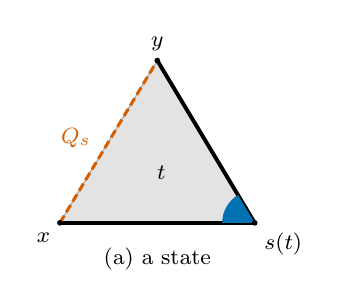
\begin{tikzpicture}[x=0.085\textwidth,y=0.085\textwidth,font=\footnotesize]
\coordinate (r) at (0,0); \coordinate (s) at (2.4,0); \coordinate (u) at (1.2,2);
\fill[gray!22] (r)--(s)--(u)--cycle;
\draw[gray!70] (r)--(s)--(u)--cycle;
\draw[black, line width=1.4pt] (r)--(s); \draw[black, line width=1.4pt] (s)--(u);
\draw[rorange, line width=1.1pt, dash pattern=on 3pt off 1.5pt] (r)--(u);
\fill[sblue] (s) -- ++(180:0.4) arc[start angle=180, delta angle=-59, radius=0.4] -- cycle;
\fill (r) circle (0.035); \fill (s) circle (0.035); \fill (u) circle (0.035);
\node[below left] at (r) {$x$}; \node[below right] at (s) {$s(t)$}; \node[above] at (u) {$y$};
\node at (1.25,0.62) {$t$};
\node[rorange, left] at (0.5,1.05) {$Q_s$};
\node at (1.2,-0.45) {(a) a state};
\end{tikzpicture}\hfill
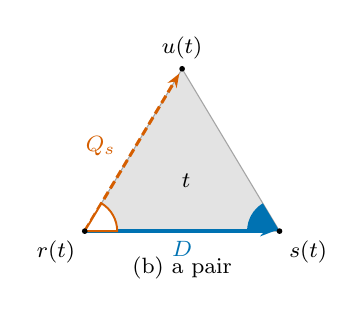
\begin{tikzpicture}[x=0.085\textwidth,y=0.085\textwidth,font=\footnotesize]
\coordinate (r) at (0,0); \coordinate (s) at (2.4,0); \coordinate (u) at (1.2,2);
\fill[gray!22] (r)--(s)--(u)--cycle;
\draw[gray!70] (r)--(s)--(u)--cycle;
\draw[sblue, line width=1.2pt, -{Stealth[length=5pt]}, shorten >=2pt] (r)--(s);
\draw[rorange, line width=1.1pt, dash pattern=on 3pt off 1.5pt, -{Stealth[length=5pt]}, shorten >=2pt] (r)--(u);
\fill[sblue] (s) -- ++(180:0.4) arc[start angle=180, delta angle=-59, radius=0.4] -- cycle;
\draw[rorange, fill=white, line width=0.7pt] (r) -- ++(0:0.4) arc[start angle=0, delta angle=59, radius=0.4] -- cycle;
\fill (r) circle (0.035); \fill (s) circle (0.035); \fill (u) circle (0.035);
\node[below left] at (r) {$r(t)$}; \node[below right] at (s) {$s(t)$}; \node[above] at (u) {$u(t)$};
\node at (1.25,0.62) {$t$};
\node[sblue, below] at (1.2,0) {$\Dc$};
\node[rorange, left] at (0.5,1.05) {$Q_s$};
\node at (1.2,-0.45) {(b) a pair};
\end{tikzpicture}\hfill
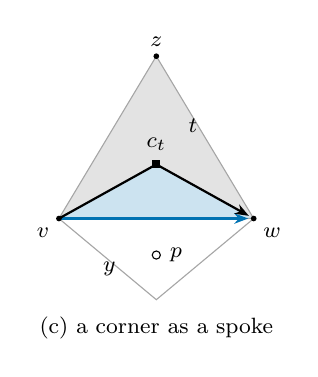
\begin{tikzpicture}[x=0.085\textwidth,y=0.085\textwidth,font=\footnotesize]
\coordinate (v) at (0,0); \coordinate (w) at (2.4,0); \coordinate (z) at (1.2,2); \coordinate (c) at (1.2,0.667);
\fill[gray!22] (v)--(w)--(z)--cycle;
\fill[sblue!20] (v)--(c)--(w)--cycle;
\draw[gray!70] (v)--(w)--(z)--cycle;
\draw[gray!70] (v)--(1.2,-1.0)--(w);
\draw[sblue, line width=1.1pt, -{Stealth[length=5pt]}, shorten >=2pt] (v)--(w);
\draw[black, line width=0.8pt, -{Stealth[length=5pt]}, shorten >=2pt] (v)--(c)--(w);
\fill[black] (1.15,0.617) rectangle (1.25,0.717);
\fill (v) circle (0.035); \fill (w) circle (0.035); \fill (z) circle (0.035);
\fill[white] (1.2,-0.45) circle (0.05); \draw (1.2,-0.45) circle (0.05);
\node[right] at (1.25,-0.45) {$p$};
\node[below left] at (v) {$v$}; \node[below right] at (w) {$w$}; \node[above] at (z) {$z$};
\node[above] at (1.2,0.72) {$c_t$};
\node at (1.65,1.15) {$t$};
\node at (0.62,-0.62) {$y$};
\node at (1.2,-1.35) {(c) a corner as a spoke};
\end{tikzpicture}
\caption{One black triangle $t$. (a) A state chooses the corner $s(t)$ (solid wedge). A selection built from $s$ may use either bold side at $s(t)$; the dashed side opposite $s(t)$ is the edge of $Q_s$ in $t$. (b) A pair adds a second corner $r(t)$ (outlined wedge). The arrow $r(t)\to s(t)$ is the edge of $\Dc(r,s)$ in $t$, and the partner directs the edge of $Q_s$ from $r(t)$ to the third corner $u(t)$. (c) The edge $v\to w$ and the route $v\to c_t\to w$ through the centre of $t$ bound the tinted region inside $t$, which contains no point $p$ of a white face such as $y$.}
\label{fig:local}
\end{figure}

\subsection*{The tree of faces}
A selection that contains $e_0$ and uses only sides at $s(t)$ in each $t\in A$ is a selection that avoids $S_s$.
It pairs each face with the face across its selected side, and those two faces are adjacent across an edge not in $S_s$.
So consider the graph $Y_s$ whose nodes are the faces of $\T$, two faces being adjacent when they share a side not in $S_s$.
In the notation of Lemma~\ref{lem:duality}, $Y_s=\T^*-S_s^*$; it is a subgraph of $G$.

\begin{lemma}\label{lem:Y}
Let $s$ be a state such that $S_s$ is a spanning tree of $\T$.
Then $Y_s$ is a tree on the $2k$ faces of $\T$, in which every face of $A$ has degree two and $t_0$ has degree one.
Root $Y_s$ at $t_0$, and let $P_s$ consist of the side that each black face shares with its child.
Then $P_s$ is a selection, $e_0\in P_s$, and for every $t\in A$ the side of $t$ in $P_s$ contains $s(t)$.
\end{lemma}

\begin{proof}
$Y_s$ is a spanning tree of the graph of faces by Lemma~\ref{lem:duality}(2).
A face $t\in A$ has exactly one side in $S_s$, its side in $Q_s$, because $ac$ and $bc$ have black face $t_0$; so $t$ has degree two in $Y_s$.
The face $t_0$ has $ac,bc\in S_s$ and $e_0\notin S_s$, so it has degree one, and its only neighbour is the white face $y_0$ across $e_0$.
Faces of $Y_s$ alternate in colour along every edge.
In the rooted tree, $t_0$ has one child, every $t\in A$ has a parent and therefore exactly one child, and every white face has a parent, which is black.
Thus every black face has exactly one side in $P_s$.
A white face $y$ is the unique child of its parent, so the side towards its parent is in $P_s$; any other side of $y$ in $P_s$ would be shared with a black child of $y$, whose child is not $y$.
So every white face has exactly one side in $P_s$ as well.
The side that $t_0$ shares with its child $y_0$ is $e_0$.
For $t\in A$ the side shared with its child is not in $Q_s$, so it is one of the two sides at $s(t)$.
\end{proof}

\begin{lemma}\label{lem:good}
For a state $s$, the set $S_s$ is a spanning tree of $\T$ if and only if $Q_s$ is a forest in which each component contains exactly one root.
\end{lemma}

\begin{proof}
$S_s$ has $|V(\T)|-1$ edges, so it is a spanning tree exactly when it is acyclic.
That happens exactly when $Q_s$ is acyclic and adding $ac$ and $bc$ closes no cycle, that is, when $a$, $b$ and $c$ lie in three different components of $Q_s$.
A forest with $n$ edges on $n+3$ vertices has three components, so this means one root in each.
\end{proof}

\begin{definition}
A state $s$ is \emph{good} if $Q_s$ is a forest in which each component contains exactly one root.
\end{definition}

Figure~\ref{fig:Q} shows a state that is good and one that is not.
For a good state, Lemma~\ref{lem:Y} produces a selection $P_s$ containing $e_0$ without any further choice.
It remains to see that $P_s$ has no cycle.
A cycle in $P_s\setminus\{e_0\}$ would be made of sides leaving chosen corners, and the next lemma says what such a cycle looks like.

\begin{figure}[t]
\centering
\includegraphics{\SHARED 09-Q.pdf}
\caption{The opposite sides $Q_s$ (dashed) for two states of the example; solid wedges mark the chosen corners, hollow circles the roots $0,4,5$. (a) This state is not good: $Q_s$ contains the triangle on the vertices $1,8,9$ around a white face. (b) This state is good: $Q_s$ is a forest with three components, each containing one root. The two states are disjoint; they form the pair of Figure~\ref{fig:pair}.}
\label{fig:Q}
\end{figure}

\subsection*{The disk identity}
Let $r$ be a state, and suppose that in every face $t\in A$ we have chosen one of the two sides at $r(t)$ and directed it out of $r(t)$.
We call these the \emph{chosen sides}.
Let $Z$ be a directed cycle of chosen sides, of length $h$.
Every vertex of $Z$ has an outgoing chosen side, so it is a vertex $r(t)$ and not a root.
The roots lie on the boundary of the outer face, so none of them lies inside $Z$ either.
Hence every face inside $Z$ is bounded, and every black face inside $Z$ is in $A$.
Let $B$ and $W$ be the numbers of black and white faces inside $Z$, let $I$ be the number of vertices strictly inside, and let $\ell$ be the number of edges of $Z$ whose black face is inside.

\begin{lemma}[disk identity]\label{lem:disk}
In this situation $W=B+1$ and $h=2\ell+3$.
In particular $h$ is odd and $Z$ encloses at least one white face.
\end{lemma}

\begin{proof}
Two of the three counts hold for every cycle of $\T$.
Euler's formula for the plane graph formed by $Z$ and everything inside it has $I+h$ vertices, $B+W+1$ faces and $(3(B+W)+h)/2$ edges, since each inner face has three sides and only the edges of $Z$ lie on a single inner face.
Signed side counting gives the second equation: count each side of an inner face with $+1$ if the face is black and $-1$ if white; an edge strictly inside contributes $+1-1$, and an edge of $Z$ contributes $+1$ or $-1$ according to its inner face.
Thus
\[
B+W=2I+h-2,\qquad 3(B-W)=2\ell-h .
\]
The third count uses the state.
Send each black face $t$ inside $Z$ to $r(t)$, a vertex inside or on $Z$.
This is injective, because $r$ is.
Every vertex $v$ strictly inside is hit: $v=r(t)$ for some $t\in A$ because $r$ is onto $X$, and $t$ has the corner $v$, so it lies inside.
A vertex $v$ on $Z$ is $r(t)$ for exactly one $t$, and the edge of $Z$ leaving $v$ is the chosen side of that $t$, because each face has only one chosen side and $r$ is injective; so $v$ is hit exactly when that edge has its black face inside.
This happens for $\ell$ vertices of $Z$, so
\[
B=I+\ell .
\]
Substituting into the first equation gives $W=I+h-\ell-2$, hence $B-W=2\ell-h+2$, and the second equation becomes $3(2\ell-h+2)=2\ell-h$, that is $h-2\ell=3$.
Then $W-B=h-2\ell-2=1$.
\end{proof}

Only the third count uses the state, and it uses both halves of bijectivity: injectivity so that no vertex is counted twice, and surjectivity so that every interior vertex is counted.
Without it the conclusion fails for directed cycles of $\T$ in general.
Figure~\ref{fig:disk} shows the counts on a cycle of the example.

\begin{figure}[t]
\centering
\includegraphics{\SHARED 08-disk.pdf}
\caption{The disk identity on a directed cycle of the example whose edges leave the corners chosen by a state $r$ (outlined wedges). The tinted disk has $B=5$ black and $W=6$ white faces, $I=3$ vertices strictly inside (ringed) and $h=7$ edges, of which $\ell=2$ have their black face inside. Each black face inside holds one outlined wedge, either at a ringed vertex or at the tail of a marked arrow, which is the count $B=I+\ell$. So $W=B+1$ and $h=2\ell+3$.}
\label{fig:disk}
\end{figure}

\subsection*{The recovered selection has no cycle}

\begin{proposition}\label{prop:recover}
If $s$ is a good state, then $P_s$ is an acyclic selection containing $e_0$.
Consequently, if $\T$ has a good state for the face $t_0$ and side $e_0$, then $G$ has a Hamiltonian cycle avoiding the edge that crosses $e_0$.
\end{proposition}

\begin{proof}
By Lemmas~\ref{lem:good} and~\ref{lem:Y}, $P_s$ is a selection containing $e_0$.
Let $P_0=P_s\setminus\{e_0\}$ and direct the side of each $t\in A$ in $P_0$ out of $s(t)$, which is one of its ends.
These are chosen sides for the state $s$ in the sense of the disk identity.
Every vertex of $X$ has outdegree exactly one, because it is $s(t)$ for exactly one $t$, and the roots have outdegree zero.

Suppose $P_0$ contains a cycle $Z$ of length $h$.
Its $h$ edges have $h$ distinct tails, all on $Z$, so every vertex of $Z$ is the tail of one of its edges and $Z$ is a directed cycle of chosen sides.
By the disk identity, $W-B=1$ and $h-2\ell=3$.
Now count the faces inside $Z$ through $P_s$.
A face inside $Z$ whose selected side is strictly inside $Z$ is matched by that side with another face inside $Z$ of the other colour.
Every edge of $Z$ lies in $P_s$, so it is the selected side of both its faces, one inside and one outside $Z$.
Thus exactly $\ell$ black faces and $h-\ell$ white faces inside $Z$ are matched across $Z$, and the rest are matched in pairs inside.
Hence $B-\ell=W-(h-\ell)$, that is $W-B=h-2\ell=3$, contradicting $W-B=1$.

So $P_0$ is a forest.
A component with $q$ vertices, of which $\alpha$ are roots, has $q-\alpha$ edges, the sum of its outdegrees, and $q-1$ edges as a tree; so $\alpha=1$.
The edge $e_0=ab$ joins the components of $a$ and $b$, so $P_s=P_0\cup\{e_0\}$ is acyclic.
The last sentence follows from Proposition~\ref{prop:target}(1).
\end{proof}

In words: a cycle of chosen sides encloses one more white face than black, but a selection running along it would force three more.

\begin{example}\label{ex:recover}
In the example, $t_0=\{0,4,5\}$, $e_0=\{0,4\}$ and $c=5$.
The state of Figure~\ref{fig:Q}(b) is good.
Figure~\ref{fig:recover}(a) shows $S_s$, its three components of $Q_s$ joined by the arcs $\{0,5\}$ and $\{4,5\}$, together with the tree of faces $Y_s$; panel (b) shows $P_s$, eleven edges forming two trees, on the vertex sets $\{0,2,4,6,7,8\}$ and $\{1,3,5,9,10,11,12\}$.
Figure~\ref{fig:selected} shows the Hamiltonian cycle of $G$ that crosses the other 22 edges.
All six good states of the example give acyclic selections in this way, and they give six different Hamiltonian cycles avoiding the edge of $G$ that crosses $e_0$; these are all such cycles of this $G$.
\end{example}

\begin{figure}[t]
\centering
\begin{tikzpicture}[x=0.04\textwidth,y=0.04\textwidth]\input{\FIG fig-recover-a}\end{tikzpicture}\hfill
\begin{tikzpicture}[x=0.04\textwidth,y=0.04\textwidth]\input{\FIG fig-recover-b}\end{tikzpicture}
\caption{Recovery from the good state of Figure~\ref{fig:Q}(b) (solid wedges). (a) The bold edges are $S_s$: the forest $Q_s$ and the two root sides other than $e_0$, here the left and right arcs. It is a spanning tree of $\T$. The dash-dotted tree $Y_s$ joins the faces across the remaining edges (squares black faces, circles white faces); $t_0$ is the leaf below the disk. (b) Rooting $Y_s$ at $t_0$, each black face selects the side it shares with its child (arrows). The bold selection $P_s$ contains $e_0$, the bottom arc, and has no cycle.}
\label{fig:recover}
\end{figure}

\begin{figure}[t]
\centering
\includegraphics{\SHARED 13-selected.pdf}
\caption{The same selection $P_s$ (bold) in the shared figure style. (a) The dash-dotted tree is $Y_s$ with its black nodes suppressed, a tree on the white faces rooted at the ringed face $y_0$ across $e_0$; each white face other than $y_0$ selects the side towards its parent. (b) The curve crossing every edge not in $P_s$ once is the Hamiltonian cycle of $G$ through all 22 faces. Its two sides hold the two components of $P_s$ (disks and squares), which are induced trees.}
\label{fig:selected}
\end{figure}

So Theorem~\ref{thm:main} follows once we find a good state, and once we can deal with triangulations in which none exists.
Section~\ref{sec:pairs} finds a good state from a pair of disjoint states, Section~\ref{sec:flow} finds a pair when $\T$ has no separating triangle, and Section~\ref{sec:glue} removes separating triangles.

\section{Pairs of states}\label{sec:pairs}

\subsection*{Why a second state}
Goodness asks two things of $Q_s$: no cycle, and one root per component.
The second condition is global and awkward to control.
A second state takes care of it.

\begin{definition}
A \emph{pair} is an ordered pair $(r,s)$ of states with $r(t)\neq s(t)$ for every $t\in A$; we call $r$ a \emph{partner} of $s$.
For a pair we write $u(t)$ for the third corner of $t$.
\end{definition}

\begin{lemma}\label{lem:partner}
Let $(r,s)$ be a pair, and direct the edge of $Q_s$ in each $t\in A$ from $r(t)$ to $u(t)$.
Then every vertex of $X$ has outdegree one and every root has outdegree zero.
Each component of $Q_s$ either is a tree containing exactly one root, or contains no root and exactly one cycle, which is directed.
In particular, $s$ is good if and only if $Q_s$ is acyclic.
\end{lemma}

\begin{proof}
The edge of $Q_s$ in $t$ joins $r(t)$ and $u(t)$, and $r$ is a bijection onto $X$, which gives the outdegrees.
A component with $q$ vertices and $\alpha$ roots has $q-\alpha$ edges, which is at least $q-1$ because it is connected.
If $\alpha=1$ it is a tree.
If $\alpha=0$ it has $q$ edges and so exactly one cycle; the edges of that cycle have distinct tails on the cycle, so every vertex of the cycle is a tail and the cycle is directed.
\end{proof}

Figure~\ref{fig:local}(b) shows the two edges that a pair gives in a black face.
Besides $Q_s$ there is $\Dc(r,s)$, the set of edges $r(t)\to s(t)$, $t\in A$.
Every vertex of $X$ is $r(t)$ for one $t$ and $s(t')$ for one $t'$, so it has one outgoing and one incoming edge in $\Dc(r,s)$.
The edges come from distinct black faces, so they are distinct even as undirected edges.
Hence $\Dc(r,s)$ is a union of disjoint directed cycles of $\T$, each of length at least three, covering $X$.
Its edges are chosen sides for the state $r$, and so are the edges of $Q_s$ directed as in Lemma~\ref{lem:partner}.
So the disk identity applies to every cycle of $\Dc(r,s)$ and to every cycle of $Q_s$.
Figure~\ref{fig:pair} shows a pair of the example.

\begin{figure}[t]
\centering
\includegraphics{\SHARED 07-pair-D.pdf}
\caption{(a) A pair of the example: outlined wedges mark $r$, solid wedges $s$. The state $s$ is the one of Figure~\ref{fig:Q}(a) and $r$ the good state of Figure~\ref{fig:Q}(b). (b) The arrows $r(t)\to s(t)$ form $\Dc(r,s)$, here a counterclockwise cycle of length $7$ through $6,1,2,3,9,10,11$ and a clockwise triangle through $8,7,12$.}
\label{fig:pair}
\end{figure}

\subsection*{Two reversals}
A pair can be changed along a cycle in two ways.

\begin{lemma}\label{lem:reversals}
Let $(r,s)$ be a pair.
\begin{enumerate}
\item Let $K$ be a cycle of $Q_s$, and put $\tilde r(t)=u(t)$ for the faces $t$ supplying $K$ and $\tilde r(t)=r(t)$ otherwise.
Then $(\tilde r,s)$ is a pair, the orientation of $K$ given by $\tilde r$ is the reverse of that given by $r$, and the same operation applied to $(\tilde r,s)$ and $K$ returns $(r,s)$.
\item Let $C$ be a cycle of $\Dc(r,s)$, and exchange $r(t)$ and $s(t)$ for the faces $t$ supplying $C$.
The result is a pair whose $\Dc$ is $\Dc(r,s)$ with $C$ reversed.
\end{enumerate}
\end{lemma}

\begin{proof}
(1) By Lemma~\ref{lem:partner} the cycle $K$ is directed by $r$, so $r$ maps the faces supplying $K$ onto the tails of its edges, which are all its vertices, and $u$ maps them onto the heads, which are again all its vertices.
So $\tilde r$ is a bijection, and $\tilde r(t)=u(t)\neq s(t)$.
In the faces of $K$ the corners $r(t)$ and $u(t)$ trade roles, so $K$ is reversed and the operation undoes itself.
(2) The tails and heads of $C$ are both its vertex set, so both new maps are bijections, and they still differ on every face.
\end{proof}

\begin{table}[ht]
\centering
\begin{tabular}{@{}llll@{}}
\toprule
reversal of & changes & keeps & cycles of $\Dc$ \\
\midrule
a cycle of $Q_s$ & $r$ on the faces of the cycle & $s$, hence $Q_s$ & may change completely\\
a cycle of $\Dc(r,s)$ & both $r$ and $s$ on its faces & the undirected edges of $\Dc$ & one cycle reversed\\
\bottomrule
\end{tabular}
\caption{The two reversals of Lemma~\ref{lem:reversals}.}
\label{tab:reversals}
\end{table}

\subsection*{A sign}
We want to count pairs so that the pairs with cyclic $Q_s$ cancel.
The reversal of a cycle of $Q_s$ pairs them up, so we need a sign that this reversal changes.
For adjacent vertices $v,w$ put $\delta(v,w)=1$ if the black face of the edge $vw$ lies to the left of $v\to w$, and $\delta(v,w)=-1$ otherwise.
Equivalently, $\delta(v,w)=1$ when $w$ follows $v$ in the counterclockwise order of the corners of that black face.
Along a directed cycle $Z$ of $\T$ traversed counterclockwise, the inside is on the left, so $\sum_{Z}\delta=\ell-(h-\ell)=2\ell-h$ in the notation of the disk identity, and the clockwise sum is $h-2\ell$.
For a directed cycle of chosen sides, the disk identity turns these into $-3$ and $+3$.
Put
\[
J(r,s)=\frac13\sum_{t\in A}\delta\bigl(r(t),s(t)\bigr).
\]

\begin{lemma}\label{lem:sign}
For every pair, $J(r,s)$ is the number of clockwise cycles of $\Dc(r,s)$ minus the number of counterclockwise ones, and $n+J(r,s)$ is even.
The sign
\[
\eps(r,s)=(-1)^{(n+J(r,s))/2}
\]
changes under both reversals of Lemma~\ref{lem:reversals}.
\end{lemma}

\begin{proof}
The sum defining $3J$ splits over the cycles of $\Dc(r,s)$, each contributing $+3$ or $-3$, which gives the first statement.
Every cycle has odd length by the disk identity, and the lengths add up to $|X|=n$, so the number of cycles is congruent to $n$ modulo $2$; it is also congruent to $J$.

Reversing a cycle of $\Dc(r,s)$ changes its contribution to $J$ from $\pm1$ to $\mp1$, so $J$ changes by $2$ and $\eps$ changes sign.
For a cycle $K$ of $Q_s$, look at a face $t$ supplying $K$.
Its corners in counterclockwise order are $r(t),s(t),u(t)$ or $r(t),u(t),s(t)$.
In the first case $\delta(r,s)=1$, $\delta(u,s)=-1$ and $\delta(r,u)=-1$; in the second all three signs flip.
In both cases
\[
\delta\bigl(u(t),s(t)\bigr)-\delta\bigl(r(t),s(t)\bigr)=2\,\delta\bigl(r(t),u(t)\bigr).
\]
Summing over the faces of $K$, the change of $3J$ is twice the $\delta$-sum of $K$ directed from $r(t)$ to $u(t)$, which is $\pm3$ by the disk identity.
So $J$ changes by $\pm2$ and $\eps$ changes sign.
\end{proof}

The reversal of a cycle of $Q_s$ can rearrange the cycles of $\Dc$ completely, so a sign defined by counting cycles alone would not be controlled.
The local formula for $J$ is what makes the change computable, and the disk identity is what makes it $\pm2$.

\subsection*{Cancellation}

\begin{lemma}\label{lem:cancel}
Let $s$ be a state for which $Q_s$ contains a cycle.
Then $\sum_r\eps(r,s)=0$, the sum running over the partners $r$ of $s$.
Consequently, for every function $F$ on states,
\[
\sum_{(r,s)\ \text{pair}}\eps(r,s)\,F(s)=\sum_{s\ \text{good}}F(s)\sum_{r}\eps(r,s).
\]
\end{lemma}

\begin{proof}
Fix an order on the cycles of $\T$, and let $K_s$ be the first cycle of $Q_s$; it depends on $s$ only.
For a partner $r$ of $s$, reverse $K_s$ as in Lemma~\ref{lem:reversals}(1).
The new partner $\tilde r$ has the same second state $s$, so the same $Q_s$ and the same $K_s$, and reversing again gives back $r$.
This is an involution on the partners of $s$ without fixed points, and by Lemma~\ref{lem:sign} it changes $\eps$.
So the sum is zero.
For the second statement, group the pairs by $s$; the states with a partner and acyclic $Q_s$ are the good states by Lemma~\ref{lem:partner}.
\end{proof}

The cycle $K_s$ must be chosen from $s$ alone; a choice that looked at $r$ might pick a different cycle after the reversal, and the map would not be an involution.
Figure~\ref{fig:cancel} shows the one cancelling pair of the example.

\begin{figure}[t]
\centering
\begin{tikzpicture}[x=0.04\textwidth,y=0.04\textwidth]\input{\FIG fig-cancel-a}
\node[font=\footnotesize] at (0,-6.4) {(a) $(r,s)$: $J=0$, $\eps=-1$};\end{tikzpicture}\hfill
\begin{tikzpicture}[x=0.04\textwidth,y=0.04\textwidth]\input{\FIG fig-cancel-b}
\node[font=\footnotesize] at (0,-6.4) {(b) $(\tilde r,s)$: $J=-2$, $\eps=+1$};\end{tikzpicture}
\caption{Cancellation in the example ($n=10$). (a) The pair $(r,s)$ of Figure~\ref{fig:pair}; dashed edges are $Q_s$, which contains the triangle on $1,8,9$ (tinted inside). The partner $r$ (outlined wedges) directs it counterclockwise. (b) Reversing that triangle moves the outlined wedges in its three faces to the third corners and leaves the solid wedges, the state $s$, unchanged. The sign changes, so the two pairs cancel in any sum weighted by a function of $s$.}
\label{fig:cancel}
\end{figure}

\subsection*{Heights}
Lemma~\ref{lem:cancel} turns the search for a good state into a question: is there a function $F$ of the second state for which $\sum_{(r,s)}\eps(r,s)F(s)\neq0$?
With $F=1$ the answer is no: reversing the cycle of $\Dc(r,s)$ through a fixed vertex pairs every pair with one of opposite sign.
To break that symmetry, $F$ must distinguish the two orientations of a cycle of $\Dc$.
The disk identity offers a way: every such cycle encloses a white face.
We measure, for each white face, how often the chosen corners of $s$ wind around it.

Place a point $c_t$ inside each face $t\in A$ and call the segments from $c_t$ to the corners of $t$ \emph{spokes}; we draw the corner $(t,v)$ as the spoke $c_t v$, directed from $c_t$ to $v$.
For each white face $w$ fix a point $p_w$ inside $w$ and a polygonal path $\gamma_w$ from $p_w$ to a point $q$ in the outer face that avoids the vertices of $\T$ and the points $c_t$ and crosses spokes transversally.
For a spoke $c_t v$ let $\kappa_w(t,v)$ be the number of times it crosses $\gamma_w$ from the right of $\gamma_w$ to its left, minus the number of crossings in the other direction.
The \emph{height} of a state $s$ at $w$ and its \emph{weight} are
\[
h_s(w)=\sum_{t\in A}\kappa_w\bigl(t,s(t)\bigr),\qquad \omega(s)=\sum_{w\ \text{white}}h_s(w).
\]
Changing the paths adds to each $h_s(w)$ a constant that does not depend on $s$; nothing below depends on the choice.

\begin{lemma}\label{lem:height}
Let $(r,s)$ be a pair, $C$ a clockwise cycle of $\Dc(r,s)$, and $(r',s')$ the pair obtained by reversing $C$.
Then $h_{s'}(w)-h_s(w)$ is $1$ if $w$ lies inside $C$ and $0$ otherwise.
Hence $\omega(s')-\omega(s)=L(C)$, the number of white faces inside $C$, and $L(C)\ge1$.
\end{lemma}

\begin{proof}
After the reversal $C$ runs counterclockwise, with edges $s(t)\to r(t)$ and $s'(t)=r(t)$ on its faces.
So $h_{s'}(w)-h_s(w)=\sum_{t}\bigl(\kappa_w(t,r(t))-\kappa_w(t,s(t))\bigr)$ over the faces $t$ supplying $C$.
This is the signed number of crossings of $\gamma_w$ with the closed curve $\Gamma$ obtained from the counterclockwise cycle $C$ by replacing each edge $s(t)\to r(t)$ with the route $s(t)\to c_t\to r(t)$; the first spoke is traversed backwards, which accounts for the minus sign.
For a closed polygonal curve $\Gamma$ and a path from $p$ to $q$ in general position, the signed number of crossings, counted as above, is the winding number of $\Gamma$ around $p$ minus its winding number around $q$; the winding number changes by one each time the path crosses $\Gamma$.
Each edge of $C$ and its route lie in one closed black triangle and have the same ends (Figure~\ref{fig:local}(c)), so $\Gamma$ can be deformed into $C$ inside these triangles.
The triangles contain neither $p_w$, which lies in a white face, nor $q$, which lies in the outer face.
So $\Gamma$ and $C$ have the same winding numbers around $p_w$ and $q$.
As $C$ is a counterclockwise simple closed curve, these are $1$ or $0$ around $p_w$ according as $w$ is inside $C$ or not, and $0$ around $q$, which lies in the outer face.
Finally $L(C)\ge1$ by the disk identity.
\end{proof}

Since $h_s(w)$ is a sum over faces, and different cycles of $\Dc(r,s)$ use different faces, the effects of reversing several cycles add up.

\subsection*{The total is not zero}
Let $m\ge1$ be the smallest number of cycles of $\Dc(r,s)$ over all pairs, assuming a pair exists.
We take $F=\omega^m$.
The $m$-th power is what makes the cycles with fewest cycles count, as the following computation shows.

\begin{lemma}\label{lem:difference}
Let $b,L_1,\dots,L_c$ be real numbers and $m\ge0$ an integer.
Then
\[
\sum_{x\in\{0,1\}^c}(-1)^{x_1+\dots+x_c}\bigl(b+x_1L_1+\dots+x_cL_c\bigr)^m
=\begin{cases}0 & \text{if } c>m,\\ (-1)^c\,c!\,L_1\cdots L_c & \text{if } c=m.\end{cases}
\]
\end{lemma}

\begin{proof}
Expand the power and use $x_i^j=x_i$ for $x_i\in\{0,1\}$ and $j\ge1$.
Every term becomes a constant times $\prod_{i\in I}x_i$ for a set $I$ with $|I|\le m$.
For such a product the sum over $x$ factors into one sum for each $i$, namely $\sum_{x_i}(-1)^{x_i}x_i=-1$ if $i\in I$ and $\sum_{x_i}(-1)^{x_i}=0$ if $i\notin I$.
So it is $0$ unless $I=\{1,\dots,c\}$, and $(-1)^c$ then.
If $c>m$ no term has $I=\{1,\dots,c\}$.
If $c=m$, those terms arise by taking a different $x_iL_i$ from each of the $m$ factors, in $c!$ ways.
\end{proof}

\begin{proposition}\label{prop:good}
If $\T$ has a pair, then it has a good state.
\end{proposition}

\begin{proof}
Consider $\Sigma=\sum_{(r,s)}\eps(r,s)\,\omega(s)^m$ over all pairs.
By Lemma~\ref{lem:cancel} it is a sum over good states, so it suffices to show $\Sigma\neq0$.

Group the pairs by the undirected edge set of $\Dc(r,s)$.
Fix a pair $(r,s)$ whose $\Dc$ has cycles $C_1,\dots,C_c$, and consider any pair $(r',s')$ with the same undirected edges.
In each face $t$ it has $(r'(t),s'(t))=(r(t),s(t))$ or $(s(t),r(t))$.
Along a cycle, consecutive faces make the same choice: if exactly one of the two edges at a vertex $x$ were reversed, then $x$ would be the value of $r'$, or of $s'$, at two different faces.
So the group of $(r,s)$ consists of the $2^c$ pairs obtained by reversing some of its cycles, and these are pairs by Lemma~\ref{lem:reversals}(2).
Index them by $x\in\{0,1\}^c$, with $x_i=1$ when $C_i$ runs counterclockwise.
By Lemma~\ref{lem:sign}, $J=c-2(x_1+\dots+x_c)$, so $\eps=(-1)^{(n+c)/2}(-1)^{x_1+\dots+x_c}$.
By Lemma~\ref{lem:height}, $\omega=b+x_1L(C_1)+\dots+x_cL(C_c)$, where $b$ is the weight of the second state in the all-clockwise orientation.
By Lemma~\ref{lem:difference}, the group contributes $0$ if $c>m$, and
\[
(-1)^{(n+m)/2}(-1)^m\,m!\,L(C_1)\cdots L(C_m)=(-1)^{(n-m)/2}\,m!\,L(C_1)\cdots L(C_m)
\]
if $c=m$.
Every group has $c\ge m$, at least one has $c=m$, and every $L(C_i)\ge1$.
So
\[
\Sigma=(-1)^{(n-m)/2}\,m!\sum_{\Dc}\ \prod_{C\in\Dc}L(C)\neq0,
\]
the sum running over the undirected cycle covers with $m$ cycles.
\end{proof}

The minimum $m$ cannot be dropped: a group with $c$ cycles contributes with the sign $(-1)^{(n-c)/2}$ in its leading term, and this sign alternates as $c$ grows by two.
Only the groups with the fewest cycles are guaranteed to agree.

\begin{example}\label{ex:count}
In the example, $n=10$ and the 8 pairs fall into two groups of four.
Both have $m=2$ cycles.
In the first, a $7$-cycle encloses $L=6$ white faces and a triangle encloses $L=1$ (Figures~\ref{fig:pair} and~\ref{fig:white}); in the second, a $7$-cycle encloses $3$ white faces and a triangle $1$.
So $\Sigma=(-1)^4\,2!\,(6\cdot1+3\cdot1)=18$, which is the value of the sum computed pair by pair.
Exactly one state has a cycle in $Q_s$; its two partners are the pairs of Figure~\ref{fig:cancel} and cancel.
The other six pairs have good second states, three with $\eps=+1$ and three with $\eps=-1$.
\end{example}

\begin{figure}[t]
\centering
\begin{tikzpicture}[x=0.045\textwidth,y=0.045\textwidth]\input{\FIG fig-whitefaces}\end{tikzpicture}
\caption{The cycles of $\Dc(r,s)$ for the pair of Figure~\ref{fig:pair} and the white faces they enclose: six for the counterclockwise $7$-cycle (tinted, the darker one also inside the triangle) and one for the clockwise triangle on $8,7,12$. The dotted route through the centres of three black faces (squares) is the curve $\Gamma$ of Lemma~\ref{lem:height} for the triangle; it encloses the same white face.}
\label{fig:white}
\end{figure}

\begin{remark}
The weight $\omega$ is the weight of \cite[Section~5]{openai2026} for one particular choice of its spoke circulation: $L(C)$ is the quantity $L^+(C)-L^-(C)$ there, and our Lemma~\ref{lem:height} replaces its Lemma~5.3 and the sliding argument of its Section~5.3.
OpenAI tests the signed count against $\exp(x\,\omega(s))$ with the phase $i^{J}$ in place of $\eps$, and reads off the Taylor coefficient of order $m$; since $i^{J}=i^{-n}\eps$, that coefficient is $i^{-n}\Sigma/m!$.
The constructive paper \cite{constructive2026} uses the integer polynomial $\sum\eps(r,s)z^{\omega(s)}$ and its coefficient of $(z-1)^m$, which is again $\Sigma/m!$; Li \cite{li2026} counts lists of $m$ marks, which are the terms of $\omega(s)^m$.
The argument is not constructive; algorithms are discussed in \cite{constructive2026}.
\end{remark}

\section{The first pair}\label{sec:flow}

Proposition~\ref{prop:good} needs one pair.
Let $\mathcal{B}$ be the bipartite graph on $A\cup X$ in which $t$ is joined to its corners in $X$.
States are the perfect matchings of $\mathcal{B}$, and a pair is the same as a spanning subgraph of $\mathcal{B}$ in which every vertex has degree two: such a subgraph is a union of disjoint even cycles, and taking alternate edges along each cycle splits it into two disjoint perfect matchings.

Give the edges of a network capacity $2$ from a source to each $x\in X$, capacity $1$ from $x$ to each face $t\in A$ with corner $x$, and capacity $2$ from each $t\in A$ to a sink.
An integral flow of value $2n=2|X|=2|A|$ saturates every source and sink edge, and the incidences carrying flow form the required subgraph.
A cut with $S\subseteq X$ on the source side and the best placement of each $t$ has capacity $2(n-|S|)+\sum_{t\in A}\min\bigl(2,|V(t)\cap S|\bigr)$.
By the integral max-flow min-cut theorem \cite{fordfulkerson1956}, a pair exists if
\begin{equation}\label{eq:hall}
\sum_{t\in A}\min\bigl(2,|V(t)\cap S|\bigr)\ \ge\ 2|S|\qquad\text{for all } S\subseteq X .
\end{equation}

A \emph{separating triangle} of $\T$ is a cycle of length three with vertices strictly on both sides.

\begin{proposition}\label{prop:pair}
If $\T$ has no separating triangle, then $\T$ has a pair.
\end{proposition}

\begin{proof}
We rewrite \eqref{eq:hall} in terms of $U=V(\T)\setminus S$, which contains the roots.
Let $e(U)$ be the number of edges of $\T$ with both ends in $U$ and $b(U)$ the number of black faces, $t_0$ included, with all corners in $U$.
A face $t\in A$ with $j$ corners in $U$ contributes $\min(2,3-j)=2-\max(0,j-1)$ to the left side of \eqref{eq:hall}, and $\max(0,j-1)$ is the number of sides of $t$ with both ends in $U$, minus one if $j=3$.
Every edge has exactly one black face, and $t_0$ has three sides in $U$ and all corners in $U$, so the left side of \eqref{eq:hall} equals $2n-(e(U)-3)+(b(U)-1)$.
Since $|S|=n+3-|U|$, condition \eqref{eq:hall} becomes
\begin{equation}\label{eq:density}
e(U)-b(U)\ \le\ 2|U|-4 .
\end{equation}
The corners of a black face with all corners in $U$ are pairwise adjacent, so they lie in one component of the graph $\T[U]$ formed by the edges with both ends in $U$.
It is therefore enough to show, for each component $K$ with $p$ vertices, $m_K$ edges and $b_K$ black faces of $\T$ with all corners in $K$, that $m_K-b_K\le 2p-4$ for the component containing the roots and $m_K-b_K\le 2p$ for the others; summing gives \eqref{eq:density}.

Small components are immediate: for $p\le3$ we have $m_K\le p(p-1)/2\le 2p$.
If the root component has $p=3$, it is the triangle $abc$ with $m_K=3$, and $b_K=1$: a second face with corners $a,b,c$ would contain the same three edges, which already lie on $t_0$ and one other face each, so the cycle $abc$ would bound two faces and $\T$ would have only three vertices.
Then $m_K-b_K=2=2p-4$.

Now let $p\ge4$, and regard $K$ as a plane graph with $f$ faces; each face has a boundary walk of length $d\ge3$, a bridge being counted twice.
\emph{The faces of $K$ of length three are exactly the faces of $\T$ with all corners in $K$.}
A face of $\T$ with corners in $K$ contains no vertex or edge of $\T$, so it is a face of $K$.
Conversely, a face of length three is bounded by a triangle $xyz$ of $K$; it is a connected region with boundary $xyz$, so it is one whole side of $xyz$.
The other side contains a vertex of $K$, because $p\ge4$.
As $xyz$ is not separating, the face side contains no vertex of $\T$.
It contains no edge either, since such an edge would join two of $x,y,z$ and be parallel to a side; so it is a face of $\T$.

Let $b$ and $w$ be the numbers of black and white faces of $K$ of length three; so $b=b_K$.
Each other face $F$ of $K$, of length $d_F\ge4$, is a union of faces of $\T$; let $\beta(F)$ be the number of black ones minus the number of white ones.
Count the sides of the faces of $\T$ in $F$ with sign $+1$ for black and $-1$ for white.
An edge of $\T$ inside $F$, including edges of other components of $\T[U]$, contributes $+1-1$.
What remains are the $d_F$ sides along the boundary walk, so $3\beta(F)$ is a sum of $d_F$ terms $\pm1$.
For $d_F=4$ the sum is even and divisible by three, hence $0$; for $d_F=5$ it is odd and divisible by three, hence $\pm3$; for $d_F\ge6$, $|\beta(F)|\le d_F/3\le d_F-4$.
In all cases $|\beta(F)|\le d_F-4$.
The faces of $K$ partition the faces of $\T$, and $\T$ has as many black faces as white by \eqref{eq:counts}, so
\[
w-b=\sum_{d_F\ge4}\beta(F)\le\sum_{d_F\ge4}(d_F-4).
\]
Counting edge sides, $2m_K=3(b+w)+\sum_{d_F\ge4}d_F=4f-(b+w)+\sum_{d_F\ge4}(d_F-4)\ge4f-2b$.
With Euler's formula $p-m_K+f=2$ this gives $m_K-b\le 2p-4$.
\end{proof}

The hypothesis entered only to show that a face of $K$ of length three is a face of $\T$.
The constructive paper \cite{constructive2026} sharpens this: a pair exists exactly when no separating triangle has black faces along all three of its sides on the side away from $t_0$.
We do not need this, because Section~\ref{sec:glue} removes all separating triangles.

\section{Separating triangles}\label{sec:glue}

Let $\Delta=xyz$ be a separating triangle of a coloured triangulation $\T$, and let $\mathsf{D}$ be one of the two closed disks it bounds.
The \emph{piece} $\T_{\mathsf{D}}$ consists of the vertices, edges and faces of $\T$ in $\mathsf{D}$, together with one new face, the \emph{cap}, bounded by $\Delta$ on the other side.

\begin{lemma}\label{lem:cap}
The three faces of $\T$ in $\mathsf{D}$ that have a side on $\Delta$ have the same colour.
Colouring the cap with the other colour makes $\T_{\mathsf{D}}$ a coloured triangulation with fewer vertices than $\T$.
\end{lemma}

\begin{proof}
Count the sides of the faces of $\T$ in $\mathsf{D}$ with sign $+1$ for black and $-1$ for white.
Edges inside $\mathsf{D}$ cancel, so three times the number of black faces minus white faces in $\mathsf{D}$ is a sum of three terms $\pm1$, one for each side of $\Delta$.
Being divisible by three, it is $\pm3$, so the three terms agree.
The piece is a triangulation of the sphere whose graph is a subgraph of $\T$, hence simple; it has a vertex strictly inside $\mathsf{D}$, so at least four vertices, and it misses the vertices strictly on the other side.
With the cap coloured oppositely, every edge of $\Delta$ has faces of both colours, and the other edges keep their two faces.
\end{proof}

\begin{theorem}\label{thm:T}
Let $\T$ be a coloured triangulation, $t_0$ a face of $\T$ and $e_0$ a side of $t_0$.
Then $\T$ has an acyclic selection containing $e_0$.
\end{theorem}

\begin{proof}
We use induction on the number of vertices.
If $\T$ has no separating triangle, exchange the colours if necessary so that $t_0$ is black.
Then $\T$ has a pair by Proposition~\ref{prop:pair}, a good state by Proposition~\ref{prop:good}, and an acyclic selection containing $e_0$ by Proposition~\ref{prop:recover}.

Otherwise let $\Delta=xyz$ be a separating triangle.
Let $\mathsf{D}_1$ be the closed disk bounded by $\Delta$ that contains $t_0$, let $\mathsf{D}_2$ be the other, and let $\T_1,\T_2$ be the pieces, coloured as in Lemma~\ref{lem:cap}.
The face $t_0$ is a face of $\T_1$.
By induction $\T_1$ has an acyclic selection $P_1$ containing $e_0$.
The cap of $\T_1$ is bounded by $\Delta$, so $P_1$ contains exactly one side of $\Delta$; call it $e'$.
The cap of $\T_2$ is also bounded by $\Delta$, and by induction $\T_2$ has an acyclic selection $P_2$ containing $e'$, which is then its only side of $\Delta$.
Put $P=P_1\cup P_2$.

\emph{$P$ is a selection containing $e_0$.}
Every face of $\T$ other than the caps is a face of exactly one piece; say $f$ is a face of $\T_1$.
The edges that $\T_1$ and $\T_2$ share are the sides of $\Delta$, and $P_2$ contains only $e'$ among them, which is also in $P_1$.
So $f$ has the same sides in $P$ as in $P_1$, namely exactly one.
The same holds for faces of $\T_2$.

\emph{$P$ is acyclic.}
By Proposition~\ref{prop:target}(2) applied in $\T_i$, an edge of $\Delta$ other than $e'$ has its ends in different components of $P_i$.
So if $e'=xy$, then $x$ and $y$ lie in one component of $P_i$ and $z$ in the other, and the only path in $P_i$ between two of $x,y,z$ is the edge $e'$ itself.
Suppose $Z$ is a cycle in $P$.
It is not contained in $P_1$ or in $P_2$, so it contains an edge of $P_2\setminus P_1$, which is not a side of $\Delta$ and so has an end strictly inside $\mathsf{D}_2$.
Follow $Z$ from this edge in both directions until it first meets $\{x,y,z\}$.
The pieces meet only in $x,y,z$, so this gives a path in $P_2$ of length at least two between two vertices of $\{x,y,z\}$, and these two vertices are distinct because $Z$ is not contained in $P_2$.
This contradicts the previous paragraph.
\end{proof}

Read in the primal graph, $\Delta$ is a cut of three edges, each piece is $G$ with one side of the cut contracted to a vertex, and the gluing joins two Hamiltonian cycles that use the same two cut edges; this is the form of the argument in \cite[Appendix~C]{li2026}.
The prescribed edge is what makes the gluing work: $P_2$ must use the same side of $\Delta$ as $P_1$, and an arbitrary acyclic selection of $\T_2$ need not.
Figure~\ref{fig:glue} shows a small case.

\begin{figure}[t]
\centering
\includegraphics{\SHARED 14-gluing.pdf}
\caption{Gluing across the separating triangle $\{3,4,5\}$ of an octahedron with a second octahedron inside one face. (a) The outer piece, its cap tinted; its acyclic selection (bold) uses the side $\{3,5\}$ of the cap. (b) The inner piece with the cap as its outer face and $\{3,5\}$ prescribed. (c) The union is an acyclic selection of the whole triangulation. Disks and squares mark the two components.}
\label{fig:glue}
\end{figure}

\begin{proof}[Proof of Theorem~\ref{thm:main}]
By Lemma~\ref{lem:dual}, the dual $\T$ of $G$ is a coloured triangulation.
Let $e_0$ be the edge of $\T$ crossing $e$ and $t_0$ one of its two faces.
Theorem~\ref{thm:T} gives an acyclic selection $P$ with $e_0\in P$, and by Proposition~\ref{prop:target}(1) the edges of $G$ not in $P^*$ form a Hamiltonian cycle.
It avoids $e$, because $e\in P^*$.
\end{proof}

\section{What each hypothesis does}\label{sec:hyp}

\emph{Bipartite.}
The colouring of the faces of $\T$ is the bipartition of $G$.
It gives every edge exactly one black face, which makes $Q_s$ and $\Dc(r,s)$ consist of distinct edges and gives the counts \eqref{eq:counts}, hence $|A|=|X|$; without $|A|=|X|$ there are no states at all.
Tutte's 46-vertex graph \cite{tutte1946} is cubic, planar and 3-connected but neither bipartite nor Hamiltonian.

\emph{Cubic.}
Cubicity makes the faces of $\T$ triangles, so that a corner has a unique opposite side, and it makes the complement of a selection have degree two.

\emph{Planar.}
For a coloured triangulation of an orientable surface of genus $g$, the same counting gives $|V|=k+2-2g$, so $|X|=|A|-2g$ and there are no states when $g>0$.
Planarity is also used through the Jordan curve theorem in Lemma~\ref{lem:duality}, the disk identity and the heights.

\emph{3-connected.}
It is used once, to make $\T$ simple (Lemma~\ref{lem:dual}).
Simplicity is used in the density bound, where a face of $K$ of length two would break $|\beta(F)|\le d_F-4$, and in the pieces of Section~\ref{sec:glue}.
The hypothesis cannot be dropped from Theorem~\ref{thm:main}.
Take two new vertices and three copies of the cube with one edge removed, and join the two ends of the removed edge in each copy to the two new vertices, one to each, respecting the bipartition.
The result is cubic, bipartite, planar and 2-connected, but deleting the two new vertices leaves three components, which a Hamiltonian cycle minus two vertices cannot do.

\emph{The prescribed edge.}
It is not needed for Hamiltonicity of a triangulation without separating triangles, but the induction of Section~\ref{sec:glue} needs it for the second piece.

\emph{Not every Hamiltonian cycle arises.}
Proposition~\ref{prop:recover} turns good states into Hamiltonian cycles avoiding the edge crossing $e_0$, and different good states give different cycles, since Lemma~\ref{lem:selections-give-states} recovers $s$ from $P_s$.
In the example all six such cycles arise.
For the hexagonal prism, whose dual is the hexagonal bipyramid, a direct check with a black face as $t_0$ gives three states, two of them good, and four Hamiltonian cycles avoiding the edge; so the map is not onto in general.
The state that Lemma~\ref{lem:selections-give-states} assigns to the other two cycles has no partner.

\bibliographystyle{amsplain}
\bibliography{refs}

\end{document}
